\section{Design and Implementation}
\label{sec.design}

Designing an implementation of the popular paths metric for use with containers required completion of two separate tasks. 
First, we had to find the popular paths for the underlying host operating system. 
And, second, once we knew where these paths were, we needed a way to log / block the unpopular paths to warn and keep containers away from these less-used and potentially buggy code paths. 
Our solution was a dual module approach we call the Secure Logging System (Shown in Figure \ref{fig:design}). 

\subsection{Design of Our ``Secure Logging System''}
\label{sec.design.secure_logging_system}
Identifying the popular paths for the given container system is handled by the system module we refer to as the Kernel Profiler. 
This module identifies the lines of code in the host kernel that are executed when running its default / regular workload. 
Such a workload is often defined in the configuration files (Dockerfiles) that come with the container images. 
We collected  ``popular paths kernel traces,'' as we named them, from a set of the containers, as  ranked ``most popular'' by the number of user downloads. 

\begin{figure*}
\centering
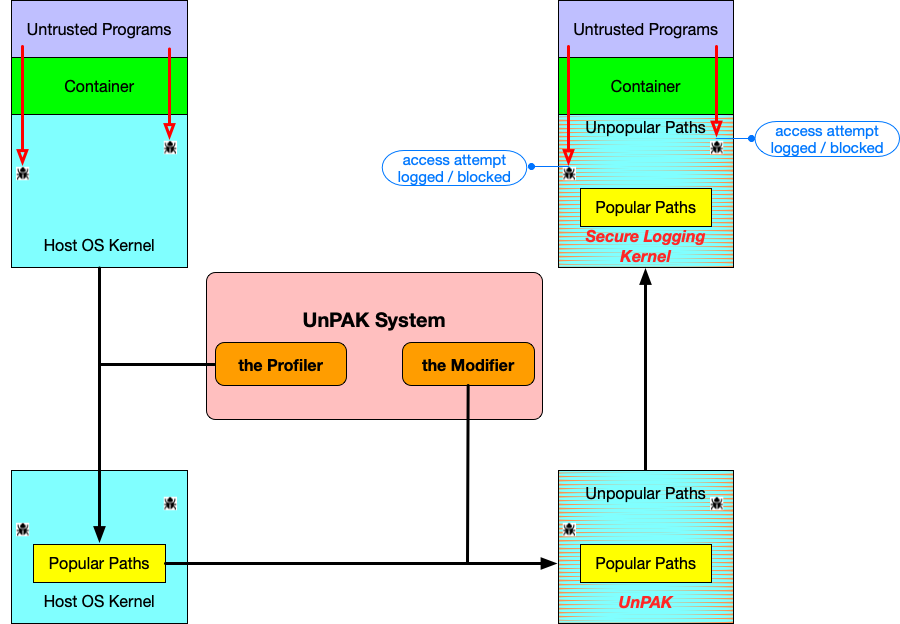
\includegraphics[width=1.5\columnwidth]{diagram/design.png}
\caption{\small Design overview of our Secure Logging System}
\label{fig:design}
\end{figure*}

In effect, the Profiler sets out a map highlighting places in the kernel that are safe for an application to access. 
The second module, the Kernel Modifier,  uses this map to instrument the rarely used unpopular paths to either generate security warning messages / logs, or to block code execution on these paths. 
When both modules are implemented, the result is an instrumented Linux kernel with security monitors and checks inserted at the non-popular paths. 
This Secure Logging Kernel can then be used to run containers without any required changes to the containers themselves.

\subsection{Implementation}
\label{sec.design.implementation}
To adapt our design for real-world containers and applications, it was necessary to build our own infrastructure to first systematically profile popular containers to obtain the popular paths data, and then use it to instrument the host Linux kernel to add the function of generating security logs and warning messages.  
This section describes in detail how the modules in our system were implemented.

\subsubsection{Implementing the Kernel Profiler}
\label{sec.design.implementation.kernel_profiler}
The Kernel Profiler is designed to collect the kernel trace of running user containers. 
The popular paths kernel trace we are looking to identify refers to the lines of code in the underlying host operating system kernel that were executed when running the regular container workload. 
This workload is defined in the configuration files of the corresponding images from containers we labeled popular based on the number of user downloads. 
Our Kernel Profiler works in the following way: 
\begin{enumerate}
	\item The Linux kernel used to run the Docker containers is recompiled with the Gcov \cite{gcov} kernel profiling feature enabled. 
	\item To run the Docker containers, the Kernel Profiler first automatically generates the configuration file for the Gcov-enabled LinuxKit. 
	This file will define a task container, running the main testing workload, along with a data container responsible for collecting, storing, and transferring the kernel trace data. 
	(shown in Figure \ref{fig:linuxkit-kernel-profiler})
	\item When booting the LinuxKit virtual machine, a script in the profiler automatically starts running the workload of the task container. 
	The profiler will collect the kernel trace data, in the form of gcda files generated by Gcov, store them at ``/sys/kernel/debug/gcov/,'' 
	and by the end of the run transfer the data from inside of the data container to the host system for further use. 
	\item Using the lcov \cite{lcov} tool to process the kernel trace data collected from the host system, the profiler generates formatted data about which lines of code were executed in the kernel source files. 
	These files will be used by the  Kernel Modifier to identify the unpopular paths that must trigger an alert if used. 
\end{enumerate}

\begin{figure*}
\centering
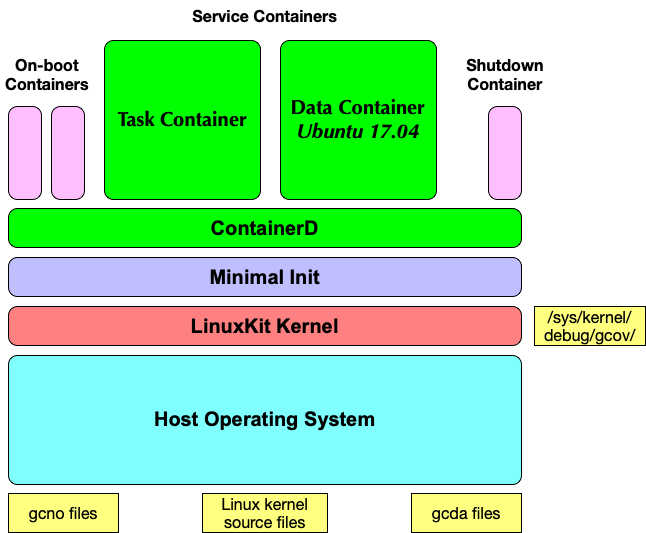
\includegraphics[width=1.5\columnwidth]{diagram/linuxkit-kernel-profiler.png}
\caption{\small Implementation of the Kernel Profiler}
\label{fig:linuxkit-kernel-profiler}
\end{figure*}

\subsubsection{Implementing the Kernel Modifier}
\label{sec.design.implementation.kernel_modifier}
For the Kernel Modifier to insert security logging code at the unpopular paths in the Linux kernel, It needs to first identify the correct places in the kernel source files to be instrumented. 
It can then modify the code as needed. The Kernel Modifier has three main parts: the Clang compiler, the Clang analyzer, and the kernel instrumenting tool (Shown in Figure \ref{fig:linuxkit-kernel-modifier}).
It operates in the following way: 
\begin{enumerate}
	\item The Clang C compiler from the Clang / LLVM project \cite{llvm}, along with a BEAR \cite{bear} tool compiled the Linux kernel source. Using BEAR, 
	we can generate a compilation database containing all the compile flags and options needed for the process. 
	In turn, this database will be used by our Clang analyzer to perform source code parsing in the next step.
	\item Once we have the compilation database for the Linux kernel,  we use the Clang analyzer to perform static analysis on the kernel source code to obtain the control flow graph for each function in the files. 
	The analyzer leveraged Clang’s LibTooling \cite{clang-libtooling} to construct the AST tree from the kernel source code, and then obtain the control flow graph. 
	With this graph, we can identify the corresponding source line number for each basic block. Furthermore, the beginning lines of all the blocks in the source files are candidates for places to add security logging code. 
	Here, a basic block refers to a straight-line code sequence with no branches in except to the entry and no branches out except at the exit. 
	Thus, if a basic block is unpopular, it is sufficient to insert only one piece of secure logging code at the beginning of it to monitor and warn the attempt to reach that code. 
	This approach can optimize our instrumentation by  avoiding redundancy in our code injection.  
	\item The next steps has the kernel instrumenting tool executing modifications based on both the basic blocks, and the collected popular paths data . 
	The algorithm for our kernel modification directs us through the basic blocks in the kernel source files. If none of the lines in a block are in the popular paths data, we consider this an unpopular basic block, 
	and our instrumenting tool will add the security logging code at the beginning of this block. If we discover that an entire function has no  lines in the popular paths data, we consider this an unpopular function, 
	and just add our security logging code once where it starts . This allows us to avoid adding redundant and unnecessary code. 
	The secure logging code we inserted in front of the unpopular paths was a kvm hypercall from the LinuxKit kernel into the host Linux kernel (Shown in Figure \ref{fig:kvm_hypercall}). 
	In this way, we can guarantee minimal affect on the LinuxKit kernel functionality, while still being able to generate security logging whenever unpopular paths were reached.
	\item The Kernel Modifier automatically inserts the secure logging code at the beginning of each basic block in the unpopular paths data. 
	Our kernel modification works at the source-code level. 
	The kernel source files are directly modified, and then compiled to produce the Secure Logging Kernel, which can be directly used to run Docker containers in the LinuxKit VM. 
\end{enumerate}

\begin{figure*}
\centering
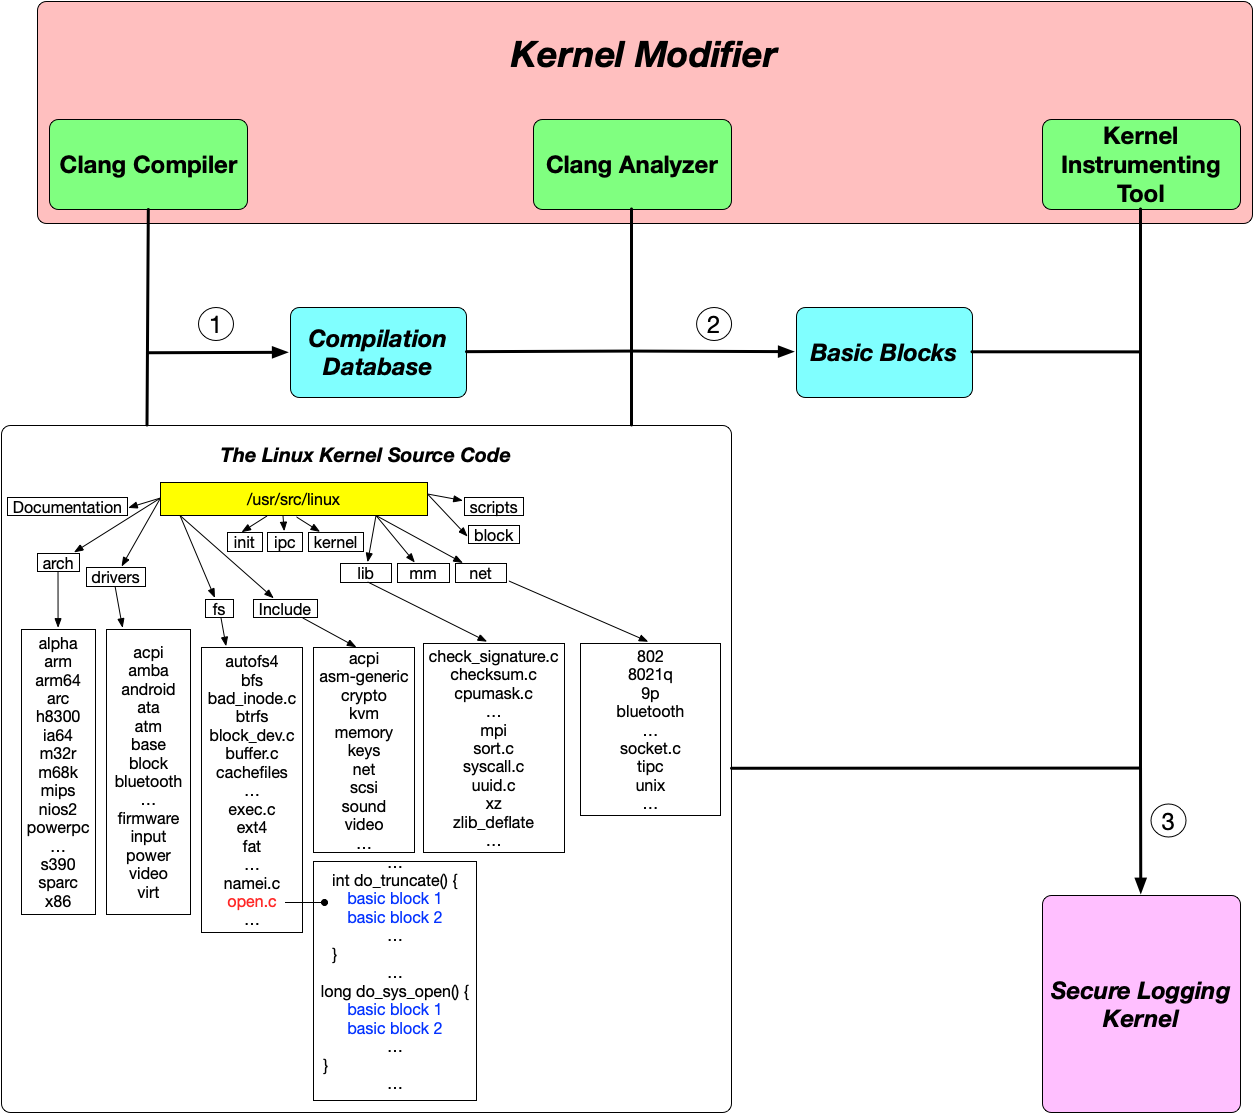
\includegraphics[width=1.5\columnwidth]{diagram/linuxkit-kernel-modifier.png}
\caption{\small Implementation of the Kernel Modifier}
\label{fig:linuxkit-kernel-modifier}
\end{figure*}

\begin{figure*}
\centering
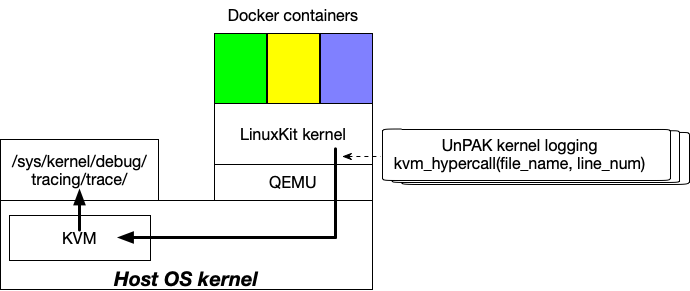
\includegraphics[width=1.5\columnwidth]{diagram/kvm_hypercall.png}
\caption{\small Our KVM\_HYPERCALL kernel instrumentation}
\label{fig:kvm_hypercall}
\end{figure*}
